\documentclass[letterpaper]{article}
\usepackage{fullpage}
\usepackage[table]{xcolor}
\usepackage{tabularx}
\usepackage{graphicx}
\usepackage{amsmath}
\usepackage{hyperref}
\usepackage{listings}
\lstset{language=python, tabsize=4}
\usepackage{tikz}
\usetikzlibrary{arrows.meta,automata,quotes,positioning,babel}

\title{Deep Learning Approach to Link Weight Prediction}

\begin{document}
\maketitle

\section{Problem}
We consider the problem of link weight prediction in a weighted directed graph.
We first take a look at a example of the problem,
and then give the problem a definition.
An undirected graph can be directly reduced to a directed graph by converting each weighted undirected link to two directed links with the same weight and opposite directions,
so the prediction for a weighted undirected graph is a special case of the problem we consider.

\subsection{Problem example}
Let us look at an example of link weight prediction - message volume prediction in a social network, shown in \autoref{fig:example} and .
In this example, there are 3 users in a social network: A, B and C.
Each user can send any amount of text messages to every other user.
We know the message size transmitted between A and C, B and C, but not A and B.
We want to predict the message size transmitted between A and B.
\begin{figure*}[!htb]\centering
	\begin{tikzpicture}[
	node distance = 80mm,
	on grid,
	> = {Stealth[length=5pt,width=4pt]},
	every state/.style = {very thick},
	every edge quotes/.style = {sloped, anchor=north}
	]
	\node[state] (B) {B};
	\node[state] (C) [below right=of B] {C};
	\node[state] (A) [above right=of C] {A};
	\path[->]   
	(A) edge[bend left,"?"]   (B)
	(B) edge[bend left,"7"]   (C)
	(B) edge[bend left,"?"]   (A)
	(A) edge[bend left,"4"]   (C)
	(C) edge[bend left,"74"]  (A)
	(C) edge[bend left,"11"]  (B);
	\end{tikzpicture}
	\caption{
		An example of link weight prediction in a weighted directed graph -
		message volume prediction in a social network.
		There are 3 users - A, B and C - in this network.
		Each user can send any amount of text messages to every other user.
		Here is what we know:
		A sent 4 messages to C,
		B sent 7 messages to C,
		and C sent 74 and 11 messages to A and B.
		Here is what we do not know and what we want to predict:
		the message volume A and B sent to each other.
		}
	\label{fig:example}
\end{figure*}
\begin{table}[!htb]\centering
	\caption{
		The same example as \autoref{fig:example}, but with edge list representation for the network.
	}
	\begin{tabularx}{\textwidth}{|X|X|c|}  \hline \rowcolor{blue!50}
		Source node & Destination node & Link weight \\ \hline
		A & B & ? \\ \hline
		A & C & 74 \\ \hline
		B & A & ? \\ \hline
		B & C & 7 \\ \hline
		C & A & 4 \\ \hline
		C & B & 11 \\ \hline
	\end{tabularx}
	\label{tab:example}
\end{table}
This is a simplified network similar to many real social networks, where every user interacts with other users by posting, sharing, following or liking them.
There can not be any logical approach to derive the unknown message volumes,
as they have randomness.
But there can be statistical approaches to build models to predict them.
The ability to predict these interactions potentially allows us to recommend new connections to users:
if A is predicted/expected to send a large amount of messages to B by some model,
and A is not connected to B yet,
we can recommend B as a new connection to A.

\subsection{Problem definition}
Now we define the link weight prediction problem in a weighted directed graph.
\begin{itemize}
	\item Given the edge list of a weighted directed graph with some unknown link weights
	\item Predict unknown link weights
\end{itemize}
There is one thing to clarify about this definition.
For every possible link (1 out of $ n^2 $, where n is the number of nodes), 
if we know its weight, we know it exists;
if we do not know its weight, we do not know it exists.
This is a very practical point when we handle streaming graphs:
for any possible link,
we either know it exists and know its weight (if it has been streamed in), or not - we never know some link does not exist or does not have weight.

\section{Baseline approaches}
In our literature study, we found very limited existing approaches to this problem.
A few approaches were derived from the SBM (Stochastic Block Model) \cite{aicher2014learning} and we use these as baseline approaches.
Now we review the SBM and its derivatives.

\subsection{SBM (Stochastic Block Model)}
The SBM is designed for unweighted graph.
The main idea is to partition nodes into K groups and connect groups with bundles.
In this way, the graph has a 2-level structure:
\begin{itemize}
	\item Lower level: each group consists of nodes which were topologically similar in the original graph
	\item Upper level: groups are connected by bundles, representing original graph
\end{itemize}
Given a graph with adjacency matrix A, the SBM has the following parameters:
\begin{itemize}
	\item A: link existence matrix, where $ A_{ij} \in \{0, 1\} $
	\item z: the group vector,
	where $ z_i \in \{ 1 ... K \} $ is the group label of node i
	\item $ \theta $: the bundle existence probability matrix,
	where $ \theta_{z_i z_j} $ is the existence probability of bundle ($z_i, z_j$)
\end{itemize}
So the existence of link (i, j) $ A_{ij} $ is a binary random variable following Bernoulli distribution:
\begin{align*}
	A_{ij} \sim B(1, \theta_{z_i z_j})
\end{align*}
The SBM fits parameters z and $ \theta $
to maximize the probability of observation A:
\begin{align*}
	P(A|z, \theta) 
	= \prod_{ij} \theta_{z_i z_j}^{A_{ij}}(1-\theta_{z_i z_j})^{1-A_{ij}}
\end{align*}
which we rewrite as log likelihood of observation A:
\begin{align*}
	\log(P(A|z, \theta))
	&= \sum_{ij} (
	{A_{ij}} \log (\theta_{z_i z_j})
	+ (1 - {A_{ij}}) \log(1-\theta_{z_i z_j})
	)\\
	&= \sum_{ij} (
	{A_{ij}} \log (\frac{\theta_{z_i z_j}}{1-\theta_{z_i z_j}})
	+ \log(1-\theta_{z_i z_j})
	)
\end{align*}
which we rewrite as an exponential family:
\begin{align*}
	\log(P(A|z, \theta))
	= \sum_{ij} (
	T(A_{ij}) \eta(\theta_{z_i z_j})
	)
\end{align*}
where
\begin{align*}
	T(x) = (x, 1)
\end{align*}
is the vector-valued function of sufficient statistics of the Bernoulli random variable and
\begin{align*}
\eta(\theta) = ( \log(\frac{\theta}{1-\theta}), \log(1-\theta) )
\end{align*}
is the vector-valued function of natural parameters of the Bernoulli random variable.

\subsection{pWSBM (pure Weighted Stochastic Block Model)}
The pWSBM is designed for weighted graph.
So it differs from SBM in a few ways described below.
Here we choose model link weight with normal distribution.
\begin{itemize}
	\item A becomes the link weight matrix so $ A_{ij} \in R $
	\item $ \theta $ becomes the bundle weight distribution parameter matrix
	so $ \theta_{z_i z_j} = (\mu_{z_i z_j}, \sigma_{z_i z_j}^2) $
	is the weight distribution parameter of bundle ($z_i, z_j$)
\end{itemize}
T(x) becomes the vector-valued function of sufficient statistics of the normal random variable:
\begin{align*}
	T(x) = (x, x^2, 1)
\end{align*}
$ \eta(\theta) $ becomes the vector-valued function of natural parameters of the normal random variable:
\begin{align*}
	\eta(\theta)
	&= \eta(\mu, \sigma^2)\\
	&= (\frac{\mu}{\sigma^2}, -\frac{1}{2\sigma^2}, -\frac{\mu^2}{2\sigma^2})
\end{align*}
So the weight of link (i, j)  $ A_{ij} $ is a real random variable following normal distribution:
\begin{align*}
	A_{ij} \sim N(\mu_{z_i z_j}, \sigma_{z_i z_j}^2)
\end{align*}
The pWSBM fits parameter z and $ \theta $
to maximize the log likelihood of observation A:
\begin{align*}
\log(P(A|z, \theta))
&= \log(P(A|z, \mu, \sigma^2))\\
&= \sum_{ij} (
A_{ij} \frac{\mu_{z_i z_j}}{\sigma_{z_i z_j}^2}
- A_{ij}^2 \frac{1}{2\sigma_{z_i z_j}^2}
- \frac{\mu_{z_i z_j}^2}{\sigma_{z_i z_j}^2}
)
\end{align*}

\subsection{bWSBM (balanced Weighted Stochastic Block Model)}

\section{Experiments}
We evaluate Model R experimentally
and the results show that 
Model R can achieve much lower prediction error than the baseline models \cite{aicher2014learning}.

\subsection{Datasets}
The experiments use 4 datasets summarized in \autoref{tab:datasets}.
\begin{table}[!htb]\centering
	\caption{The datasets used in experiments.}
	\begin{tabularx}{\textwidth}{|c|c|X|c|X|}  \hline \rowcolor{blue!50}
		Dataset & Node count & Node type & Link count & Link weight type \\ \hline
		Airport\cite{colizza2007reaction} & 500 & busiest airports in US & 5960 & number of passengers traveling from one airport to the other\\ \hline
		Collaboration\cite{pan2012world} & 226 & nations on Earth & 20616 & number of academic papers written by authors from the two connected nations \\ \hline
		Congress\cite{porter2005network} & 163  & 102nd US Congress committees & 26569 & interlock value of shared members from the two committees \\ \hline
		Forum\cite{opsahl2009clustering}  & 1899 & users of a student social network at UC Irvine & 20291 & number of messages sent from one student to the other \\ \hline
	\end{tabularx}
	\label{tab:datasets}
\end{table}

\subsection{Experiment process}
We do the same experiment for each dataset.
All the link weights are normalized to ranger [-1, 1] after applying a logarithm function.
Each experiment consists of 25 independent trials.
In each trial, we split the dataset randomly into 3 subsets:
\begin{itemize}
	\item 70\% into training set
	\item 10\% into validation set
	\item 20\% into testing set
\end{itemize}
We use mean squared error as the prediction accuracy metric.
For each experiment, we report the mean and standard deviation of the errors from 25 trials.
The pseudo code of the experiment process is as follows:

\begin{lstlisting}
	def main():
		for dataset in [Airport, Collaboration, Congress, Forum]:
			(error_mean, error_standard_deviation) = do_experiment(dataset)
	def do_experiment(dataset):
		errors = list()
		for trial in range(25):
			testing_error = append(evaluate_model_on(dataset))
			errors.append(testing_error)
		return (errors.mean(), errors.standard_deviation())
	def evaluate_model_on(dataset):
		(trainning_set, validation_set, testing_set) = split(dataset)
		while validation_error decreases:
			training_error = estimator.learn(training_set)
			validation_error = estimator.predict(validation_set)
		testing_error = estimator.predict(testing_set)
		return testing_error
\end{lstlisting}

\subsection{Experiment results}
In our experiments,
Model R's error is lower than every other model on every dataset,
shown in \autoref{fig:errors}.
\begin{figure}[!htb]\centering
	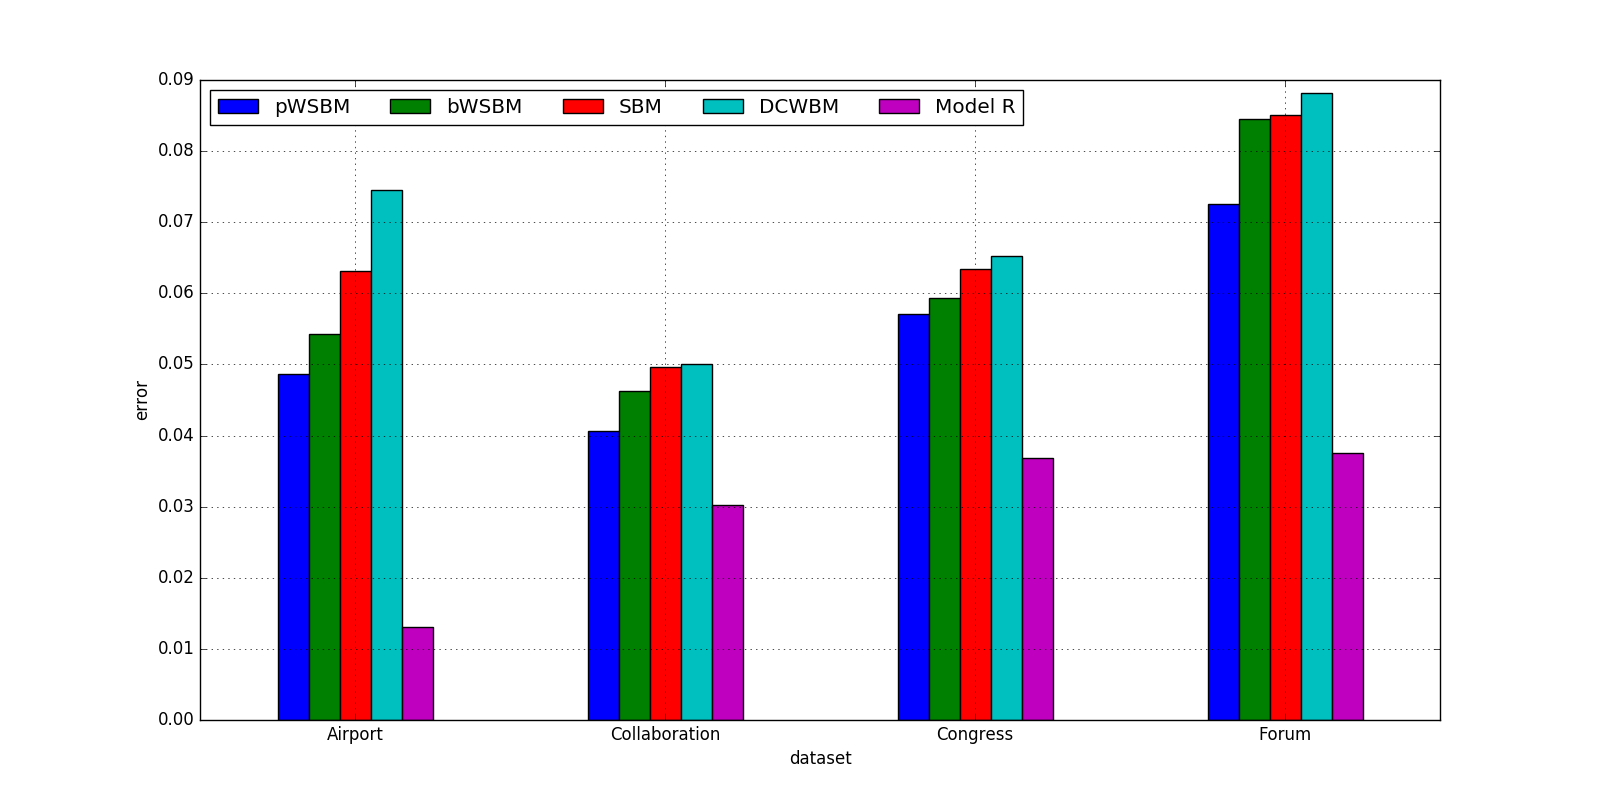
\includegraphics[width=\textwidth]{link-weight-errors}
	\caption[content...]{
		The mean squared errors of 5 models on 4 datasets:
		Model R has lower error than every other model on every dataset.
		Every error value shown here is the mean errors for the 25 trials in the experiment.
	}
	\label{fig:errors}
\end{figure}
For this section we compare Model R with only the best baseline model - pWSBM, as it outperforms other baseline models on every dataset.
Given the dataset, we regard ModelRError (or BaselineError) as a random variable so each trial generates an example of it.
We can do a t-test to justify the significance of difference between the means of variables ModelRError and BaselineError.
where $ \overline{X} $ is the mean of variable X.
The mean of a variable is not the same as the mean of a sample of the variable.
More specifically,
a variable can generate two samples with different sample means,
therefore two different sample means does not imply the two variables generating them have different means.
For each dataset, we do a t-test for the two variables where the null hypothesis is that the two variables have the same mean:
\begin{align*}
\overline{X_1} == \overline{X_2}
\end{align*}
where $ X_1 $ and $ X_2 $ are ModelRError and BaselineError.
The standard deviation $ s $ of variable X is defined as:
\begin{align*}
	s_i &= \sqrt{\overline{(X_i - \overline{X_i})^2}}
\end{align*}
Welch's t-test defines its statistic t and degrees of freedom v as:
\begin{align*}
	t &= \frac{
		\overline{X_1} - \overline{X_2}
		}{
		\sqrt{\frac{s^2_1}{N_1} + \frac{s^2_2}{N_2}}
		}\\
	v &= \frac{
		(\frac{s^2_1}{N_1} + \frac{s^2_2}{N_2})^2
		}{
		\frac{s^4_1}{N_1^2(N_1-1)} + \frac{s^4_2}{N_2^2(N_2-1)}
		}
\end{align*}
where $ N_i $ is the sample size of variable $ X_i $.
The Student's t-distribution defines its probability density function f(x) as:
\begin{align*}
f(x) = \frac{\Gamma(\frac{v+1}{2})}{\sqrt{v\pi}\Gamma(\frac{v}{2})}
((1+\frac{x^2}{v})^{-\frac{v+1}{2}})
\end{align*}
Welch's t-test defines its p value as the Student's t-distribution cumulative density function:
\begin{align*}
p = 2 \int_{-\infty}^{-|t|} f(x) dx
\end{align*}
The smaller p is, the more confidently we can reject the null hypothesis, i.e., accept that:
\begin{align*}
\overline{ModelRError} \neq \overline{BaselineError}
\end{align*}
Typically there is a domain specific threshold for p, e.g., 0.1 or 0.01. If p is smaller than the threshold we reject the null hypothesis.
We calculate the p value and also error reduction from baseline to Model R as:
\begin{align*}
Reduction = \frac{BaselineError - ModelRError}{BaselineError}
\end{align*}
The p value is almost 0 for all datasets and error reduction is significant:
ranging from 25\% on Collaboration dataset to 73\% on Airport dataset,
shown in \autoref{tab:errors}.
\begin{table}[!htb]\centering
	\caption{
		The mean squared errors of 5 models on 4 datasets:
		Model R has lower error than every other model on every dataset,
		reducing error by 25\% to 73\% from the best baseline model - pWSBM.
		The number in every parenthesis is the standard deviation of error in 25 trials in the last digit of error. The very low p values strongly indicate the error reduction is significant.
	}
	\begin{tabularx}{\textwidth}{|X|c|c|c|c|c|c|c|} \hline \rowcolor{blue!50}
		Dataset & pWSBM & bWSBM & SBM & DCWBM & Model R & Reduction & p \\ \hline
		Airport & 0.0486(6) & 0.0543(5) & 0.0632(8) & 0.0746(9) & 0.013(1) & 73\% & 4.2e-66 \\ \hline
		Collaboration & 0.0407(1) & 0.0462(1) & 0.0497(3) & 0.0500(2) & 0.030(1) & 25\% & 9.1e-44 \\ \hline
		Congress & 0.0571(4) & 0.0594(4) & 0.0634(6) & 0.0653(4) & 0.036(3) & 35\% & 7.1e-35 \\ \hline
		Forum & 0.0726(3) & 0.0845(3) & 0.0851(4) & 0.0882(4) & 0.037(1) & 48\% & 4.2e-68 \\ \hline
	\end{tabularx}
	\label{tab:errors}
\end{table}
These results show that Model R outperforms pWSBM on all these datasets.

\subsection{Computing resources}
We ran our experiments on a Lenovo ThinkCentre M83 machine with the following specifications:
\begin{itemize}
	\item Python implementation: CPython 3.5
	\item Operating system: Ubuntu 16.10 64-bit
	\item Memory: 16 GB
	\item Processor: Intel Core i7-4770 CPU @ 3.40GHz $ \times $ 8
\end{itemize}
The program - coded in Python - uses all 8 threads of the processor.
Each experiment takes about one hour to finish,
depending on the dataset and parameters in the learning algorithm.

\bibliographystyle{plain}
\bibliography{references}
\end{document}
